\documentclass{beamer}
\usepackage{graphicx}
\usepackage[T1]{fontenc}

\usetheme{Madrid}
\usecolortheme{seagull}

\title{Stepikowa Prezentacja}
\author{Jan Gasztold}
\date{\today}

\begin{document}

\begin{frame}
  \titlepage
\end{frame}

\section{Wprowadzenie}

\begin{frame}{Wstęp}
  Ta prezentacja zawiera różne treści z różnych tematyk.
  Głownie będą koty.
\end{frame}

\section{Treść}

\begin{frame}{Laptopy}
  \begin{figure}
    \centering
    
\includegraphics[width=0.7\textwidth]{image1.png}
    \caption{Koty siadają na naszych laptopach, ponieważ są w naszym centrum uwagi zamiast kotów.}
    \label{fig:rys1}
  \end{figure}
\end{frame}

\begin{frame}{Jedzenie}
  \begin{figure}[h]
    \centering
    \begin{tabular}{|c|c|c|c|c|}
        \hline
        <2 & 2-3 & 3-4 & 4-5 & 5-6 \\
        \hline
        120-160 & 160-210 & 210-260 & 240-320 & 250-360 \\
        \hline
    \end{tabular}
    \caption{Tabela jedzenia kotów.}
    \label{tab:tabela1}
\end{figure}
Tabela opisuje ile karmy powinien zjeść kot zależnie od jego masy ciała \cite{autor1}
\end{frame}

\section{Elementy Dynamiczne}

\begin{frame}{Przykładowe jedzenie którego nie mogą spożywać koty}
  \begin{itemize}
    \item Sól
    \item Mleko
    \item Owoce cytrusowe
  \end{itemize}
\end{frame}

\begin{frame}{Przykładowe jedzenie które koty powinny spożywać}
  \begin{itemize}
    \item Białko
    \item Tauryna
    \item Woda
  \end{itemize}
\end{frame}

\begin{frame}{Rasy największych kotów domowych}
  \begin{enumerate}
    \item Savannah
    \item Ashera
    \item Kot Syberyjski
  \end{enumerate}
  \begin{figure}
    \centering
    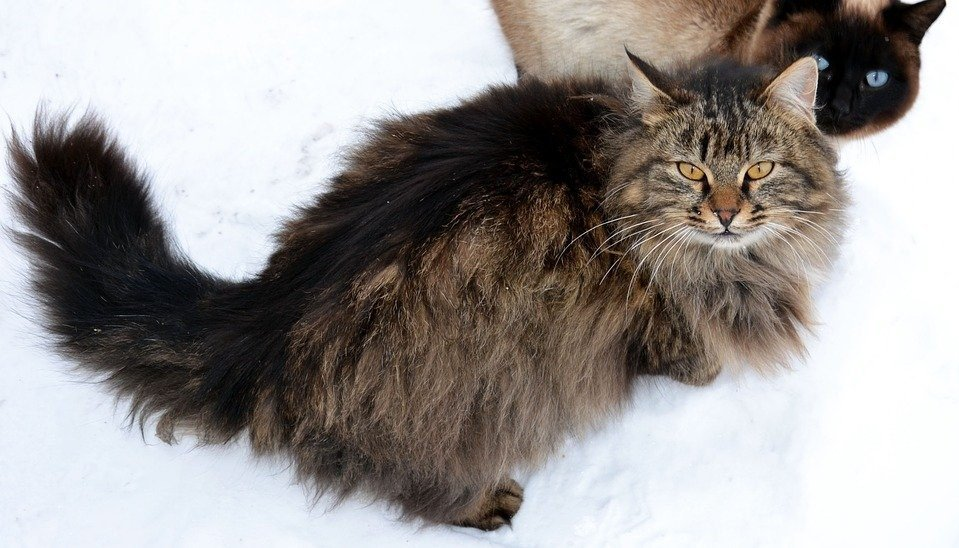
\includegraphics[width=0.7\textwidth]{image2.png}
    \caption{Kot Syberyjski}
    \label{fig:rys2}
  \end{figure}
\end{frame}

\section{Odniesienia}

\begin{frame}{Odniesienie do Rysunku}
  Koty syberyjskie Rysunek \ref{fig:rys2} pochodzą z obszarów Syberii.
\end{frame}

\begin{frame}{Odniesienie do Tabeli}
   Tabela \ref{tab:tabela1} nie jest dokładnie prawidłowa, ponieważ trzeba uwzględnić wiele innych czynników.
\end{frame}

\section{Bibliografia}

\begin{frame}{Bibliografia}
  \begin{thebibliography}{9}
    \bibitem{autor1} White, Karen. \emph{How to determine amount of Food}. Zooplus, 2015.
  \end{thebibliography}
\end{frame}

\end{document}
